\section{API REST}

\subsection{Introduction}

\begin{flushleft}
Dans cette partie, je vais vous expliquer les ajouts apportés à l'API-REST de la base du projet. 
\end{flushleft}
\begin{flushleft}
De ce fait, il me semblait plus judicieux de garder dans ce rapport que les nouvelles sections concernant mon extension.
\end{flushleft}

\subsection{Les utilisateurs invités}

\begin{flushleft}
Vous pouvez remarquer l'ajout des "Rest Services" suivants :
\end{flushleft}

\begin{enumerate}
\item \textbf{List InvitedClients} :\newline
Le GET permet de renvoyer la liste de tous les utilisateurs invités sur un portefeuille.
\item \textbf{Add InvitedClient} :\newline
Le POST permet d'ajouter un nouvel utilisateur à un portefeuille.
\item \textbf{Delete InvitedClient} :\newline
Le DELETE permet de supprimer un utilisateur invité sur un portefeuille.
\item \textbf{Change Permissions} :\newline
Le PUT permet de modifier les permissions d'un utilisateur invité.
\item \textbf{Get Permissions} :\newline
Le GET permet de renvoyer les permissions d'un utilisateur invité.
\end{enumerate}


\subsection{Les portefeuilles invités}
\begin{flushleft}
Vous pouvez également remarquer l'ajout des "Rest Services" suivants :
\end{flushleft}
\begin{enumerate}
\item \textbf{List InvitedWallets} :\newline
Le GET donne la possibilité de renvoyer la liste de tous les portefeuilles invités que possède un client.
\item \textbf{Leave InvitedWallets} :\newline
Le DELETE donne la possibilité au client de supprimer un portefeuille où il est invité.
\end{enumerate}


\newpage
\subsection{Diagramme}
\begin{figure}[h]
\centering
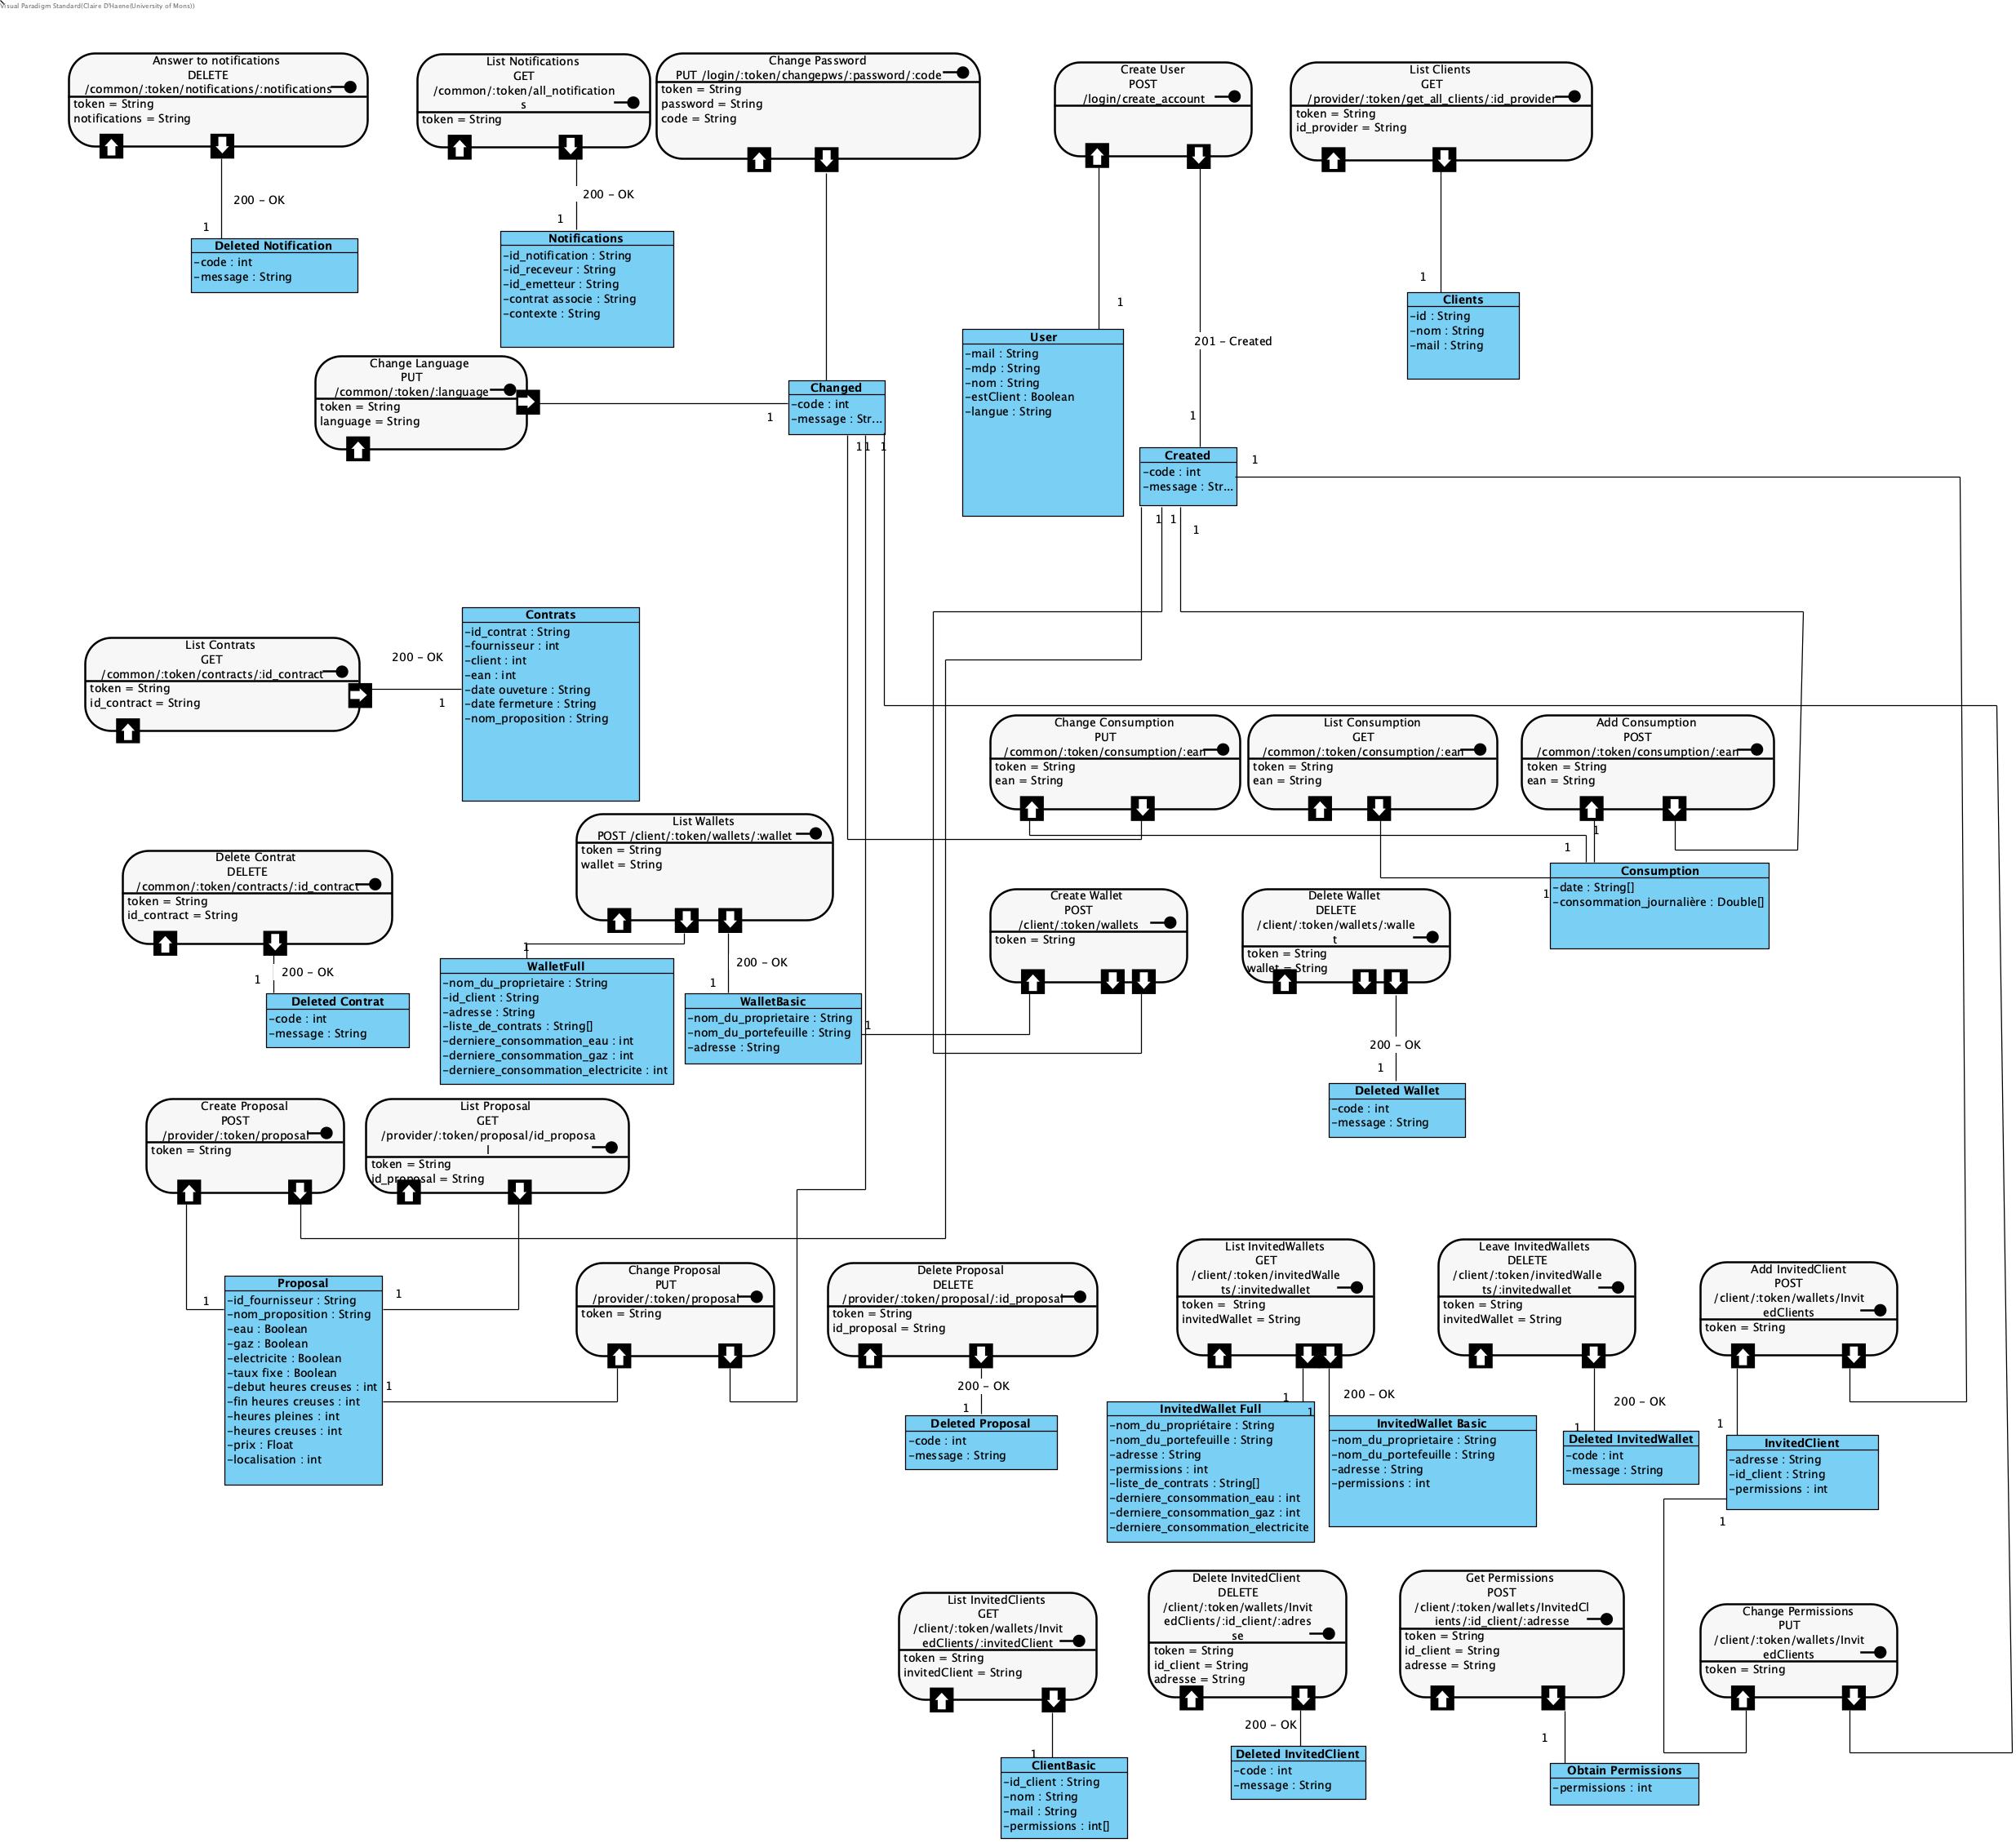
\includegraphics[width = 1\textwidth]{Extension-claire/API-claire/img/API-claire.png}
\end{figure}